\chapter{HASIL}
\label{bab:hasil}

Bab ini menyajikan hasil eksperimen klasifikasi arah XAUUSD H1 sesuai protokol Bab 3. Hasil utama menggunakan data MetaQuotes-Demo, kebijakan celah primer, dan ambang $0{,}5\sigma_{t,24}$. Hasil untuk ambang $0{,}25\sigma_{t,24}$ dan $1{,}0\sigma_{t,24}$, kebijakan \emph{holiday-reset}, serta sumber UltimaMarkets-Demo disajikan sebagai analisis sensitivitas terpisah. Angka yang dilaporkan berasal dari eksperimen Fase 4 pada 21--22 September 2026; skor uji kelayakan terdahulu tidak digunakan sebagai hasil penelitian ini.

Kinerja dilaporkan pada tujuh periode uji kronologis. Rerata skor dan perubahan antarkonfigurasi dihitung tanpa pembobotan jumlah bar, sehingga setiap periode uji mempunyai bobot sama. Penyajian menggunakan enam tempat desimal; seluruh perhitungan dilakukan dari angka sebelum pembulatan. Penafsiran hasil terhadap rumusan masalah dan keterbatasan penelitian disampaikan pada Bab 5.

\section{Hasil Audit Data dan Pembentukan Sampel}

\subsection{Cakupan Data Harga dan Celah}

Arsip harga utama berisi 38.799 bar dengan waktu pembukaan pertama 2 Januari 2020 pukul 06.00 UTC dan terakhir 31 Juli 2026 pukul 22.00 UTC. Arsip UltimaMarkets-Demo semula berisi 23.181 bar. Setelah batas awal 1 September 2022 diterapkan untuk mengecualikan lubang riwayat awal, tersisa 23.135 bar; waktu pembukaan pertama yang tersedia adalah 1 September 2022 pukul 05.00 UTC dan terakhir 31 Juli 2026 pukul 23.00 UTC. Kedua sumber dianalisis secara terpisah. Audit arsip tidak menemukan duplikasi waktu, nilai OHLC yang hilang, harga nonpositif, ataupun pelanggaran hubungan OHLC.

Tabel \ref{tab:hasil-audit-celah} merangkum klasifikasi interval antarbar yang melebihi satu jam. Penutupan terjadwal mencakup akhir pekan dan jeda sesi. Penutupan yang selaras dengan kalender bursa merupakan keselarasan antara celah teramati dan kalender bursa, dengan keterbatasan bukti historis sesi CFD broker. Kebijakan primer melanjutkan keadaan indikator setelah dua jenis penutupan tersebut. Celah tidak terjelaskan dan gangguan bursa terdokumentasi memutus keadaan indikator. Kebijakan \emph{holiday-reset} juga memutus keadaan indikator pada penutupan yang selaras dengan kalender bursa.


\begin{table}[htbp]
\centering
\small
\setlength{\tabcolsep}{4pt}
\caption{Hasil audit celah harga per sumber}
\label{tab:hasil-audit-celah}
\begin{tabular}{p{7.2cm}rr}
\toprule
Komponen & MetaQuotes & Ultima \\
\midrule
Bar setelah batas awal & 38.799 & 23.135 \\
Seluruh interval celah & 1.705 & 1.010 \\
Penutupan terjadwal & 1.627 & 965 \\
Selaras dengan kalender bursa & 69 & 44 \\
Celah tidak terjelaskan & 9 & 0 \\
Gangguan bursa terdokumentasi & 0 & 1 \\
Reset/segmen kebijakan primer & 9/10 & 1/2 \\
Reset/segmen \emph{holiday-reset} & 78/79 & 45/46 \\
\bottomrule
\end{tabular}
\end{table}


\subsection{Kelayakan Fitur, Target, dan Masker Bersama}

Sampel akhir mensyaratkan fitur yang telah melewati pemanasan, target satu bar yang sah, dan label tiga kelas yang tersedia. Tabel \ref{tab:hasil-kelayakan} menunjukkan bahwa irisan kelayakan fitur dan target pada kebijakan primer berjumlah 36.658 bar untuk MetaQuotes dan 22.031 bar untuk Ultima. Jumlah tersebut mencakup seluruh rentang data setelah penyaringan, termasuk riwayat latih; jumlah observasi uji per periode dilaporkan secara terpisah. Kebijakan \emph{holiday-reset} mengurangi sampel karena pemanasan indikator dimulai kembali pada lebih banyak celah. Bar harga tidak diinterpolasi.


\begin{table}[htbp]
\centering
\small
\setlength{\tabcolsep}{4pt}
\caption{Jumlah observasi yang memenuhi aturan kelayakan pada ambang utama}
\label{tab:hasil-kelayakan}
\begin{tabular}{llrrrr}
\toprule
Sumber & Kebijakan & Input & Fitur & Target & Irisan \\
\midrule
MetaQuotes & Primer & 38.799 & 38.342 & 36.872 & 36.658 \\
MetaQuotes & Holiday-reset & 38.799 & 35.144 & 35.318 & 33.592 \\
Ultima & Primer & 23.135 & 23.037 & 22.078 & 22.031 \\
Ultima & Holiday-reset & 23.135 & 21.052 & 21.112 & 20.128 \\
\bottomrule
\end{tabular}
\end{table}


Distribusi label pada seluruh sampel irisan ditunjukkan pada Tabel \ref{tab:hasil-distribusi-ambang}. Untuk sumber dan kebijakan yang sama, perubahan pengali ambang mengubah label tanpa mengubah jumlah bar yang memenuhi masker. Pada data utama kebijakan primer, jumlah HOLD berubah dari 9.598 menjadi 17.637 dan 27.442 ketika pengali meningkat dari 0,25 menjadi 0,50 dan 1,00. Distribusi ini dilaporkan sebagai sifat target yang dibentuk oleh protokol, bukan sebagai dasar memilih ambang berdasarkan skor model.


\begingroup
\small
\setlength{\tabcolsep}{4pt}
\begin{longtable}{llrrrrr}
\caption{Distribusi label pada seluruh sampel irisan untuk setiap pengali ambang}\label{tab:hasil-distribusi-ambang}\\
\toprule
Sumber & Kebijakan & $\alpha$ & BUY & HOLD & SELL & Jumlah \\
\midrule
\endfirsthead
\caption[]{Distribusi label pada seluruh sampel irisan untuk setiap pengali ambang (lanjutan)}\\
\toprule
Sumber & Kebijakan & $\alpha$ & BUY & HOLD & SELL & Jumlah \\
\midrule
\endhead
\midrule
\multicolumn{7}{r}{Bersambung ke halaman berikutnya} \\
\endfoot
\endlastfoot
MetaQuotes & Primer & 0,25 & 13.873 & 9.598 & 13.187 & 36.658 \\
MetaQuotes & Primer & 0,50 & 9.841 & 17.637 & 9.180 & 36.658 \\
MetaQuotes & Primer & 1,00 & 4.697 & 27.442 & 4.519 & 36.658 \\
MetaQuotes & Holiday-reset & 0,25 & 12.672 & 8.880 & 12.040 & 33.592 \\
MetaQuotes & Holiday-reset & 0,50 & 8.965 & 16.257 & 8.370 & 33.592 \\
MetaQuotes & Holiday-reset & 1,00 & 4.260 & 25.215 & 4.117 & 33.592 \\
Ultima & Primer & 0,25 & 8.297 & 5.867 & 7.867 & 22.031 \\
Ultima & Primer & 0,50 & 5.959 & 10.599 & 5.473 & 22.031 \\
Ultima & Primer & 1,00 & 2.847 & 16.475 & 2.709 & 22.031 \\
Ultima & Holiday-reset & 0,25 & 7.543 & 5.423 & 7.162 & 20.128 \\
Ultima & Holiday-reset & 0,50 & 5.394 & 9.777 & 4.957 & 20.128 \\
Ultima & Holiday-reset & 1,00 & 2.572 & 15.106 & 2.450 & 20.128 \\
\bottomrule
\end{longtable}
\endgroup


\subsection{Sampel Setiap Periode Uji}

Tabel \ref{tab:hasil-sampel-periode} memperlihatkan jumlah observasi latih setelah \emph{purge}, jumlah observasi uji, dan distribusi kelas uji untuk kebijakan primer serta ambang utama. Seluruh periode memiliki tiga kelas benar pada sampel uji. Pada MetaQuotes, ketujuh periode memenuhi persyaratan validasi internal. Total observasi uji MetaQuotes adalah 19.898 bar, dengan setiap bar dipakai bersama oleh K1, K2, K3, serta kedua model. Jumlah latih meningkat seiring bergesernya periode uji; jumlah latih tidak harus sama dengan penjumlahan sederhana jumlah uji yang ditampilkan karena kelayakan horizon label diperiksa ulang pada setiap batas periode.

Pada Ultima, tersedianya bar uji pada tiga periode awal belum mencukupi persyaratan pelatihan: riwayat sebelum September 2022 tidak tersedia untuk membentuk tiga blok validasi internal dalam 18 bulan terakhir. Oleh karena itu, K1, K2, dan K3 pada 2023-H1, 2023-H2, dan 2024-H1 berstatus \textbf{NOT TESTED} untuk kedua model. Empat periode dari 2024-H2 sampai Januari--Juli 2026 dapat dievaluasi. Periode yang gagal tetap menjadi bagian dari tujuh periode terjadwal dan tidak diberi skor rekaan.


\begingroup
\small
\setlength{\tabcolsep}{4pt}
\begin{longtable}{llrrrrr}
\caption{Sampel kebijakan primer dan ambang utama per periode uji}\label{tab:hasil-sampel-periode}\\
\toprule
Sumber & Periode & Latih & Uji & BUY & HOLD & SELL \\
\midrule
\endfirsthead
\caption[]{Sampel kebijakan primer dan ambang utama per periode uji (lanjutan)}\\
\toprule
Sumber & Periode & Latih & Uji & BUY & HOLD & SELL \\
\midrule
\endhead
\midrule
\multicolumn{7}{r}{Bersambung ke halaman berikutnya} \\
\endfoot
\endlastfoot
MetaQuotes & 2023-H1 & 16.756 & 2.807 & 699 & 1.410 & 698 \\
MetaQuotes & 2023-H2 & 19.563 & 2.829 & 669 & 1.470 & 690 \\
MetaQuotes & 2024-H1 & 22.393 & 2.808 & 740 & 1.385 & 683 \\
MetaQuotes & 2024-H2 & 25.201 & 2.870 & 830 & 1.380 & 660 \\
MetaQuotes & 2025-H1 & 28.071 & 2.735 & 816 & 1.229 & 690 \\
MetaQuotes & 2025-H2 & 30.807 & 2.746 & 838 & 1.219 & 689 \\
MetaQuotes & 2026 Jan--Jul & 33.554 & 3.103 & 809 & 1.501 & 793 \\
Ultima & 2023-H1 & 1.834 & 2.807 & 698 & 1.408 & 701 \\
Ultima & 2023-H2 & 4.641 & 2.829 & 673 & 1.467 & 689 \\
Ultima & 2024-H1 & 7.471 & 2.806 & 734 & 1.390 & 682 \\
Ultima & 2024-H2 & 10.277 & 2.868 & 825 & 1.389 & 654 \\
Ultima & 2025-H1 & 13.145 & 2.784 & 835 & 1.252 & 697 \\
Ultima & 2025-H2 & 15.930 & 2.813 & 851 & 1.246 & 716 \\
Ultima & 2026 Jan--Jul & 18.744 & 3.285 & 852 & 1.569 & 864 \\
\bottomrule
\end{longtable}
\endgroup


\section{Hasil Audit Kalender Makroekonomi}

Snapshot kalender ekonomi berisi 706 peristiwa USD pada Januari 2020--Juli 2026 tanpa duplikasi pengenal nilai. Sebanyak 520 baris mempunyai nilai aktual dan 460 baris mempunyai prakiraan. Rinciannya adalah 310 peristiwa CPI, 78 NFP, 78 tingkat pengangguran, 54 keputusan suku bunga, dan 186 peristiwa FOMC. Empat jenis CPI dipertahankan sebagai keluarga fitur terpisah. Dengan NFP dan tingkat pengangguran, terdapat enam keluarga numerik untuk kejutan aktual dikurangi prakiraan. Keputusan suku bunga dan FOMC hanya menyumbang representasi kejadian pascarilis karena prakiraan tidak tersedia.

Pemeriksaan hash memastikan snapshot kalender sama dengan arsip beku. Penandaan UTC khusus snapshot ini cocok dengan sepuluh jangkar rilis resmi lintas musim DST dan non-DST. Pada tujuh periode utama, keenam keluarga numerik mempunyai cakupan nilai kejutan pada data latih dan uji. Penggabungan kalender menggunakan rilis yang waktunya lebih awal secara ketat daripada waktu keputusan bar; rilis tepat pada waktu keputusan baru tersedia bagi keputusan berikutnya. Nilai makro yang tidak tersedia diproses dengan parameter imputasi yang dipelajari hanya dari data latih.

Hasil pemeriksaan tersebut memungkinkan K3 dilaksanakan sesuai asumsi operasional Bab 3. Riwayat independen mengenai nilai aktual rilis pertama dan prakiraan pra-rilis tidak tersedia. Karena itu, hasil K3 dalam bab ini berlaku untuk snapshot retrospektif yang dibekukan dan tidak diklaim sebagai arsip \emph{point-in-time} penuh. Validasi timestamp tidak menghapus keterbatasan versi nilai historis tersebut.

\section{Hasil Pemodelan pada Data Utama}

\subsection{Kinerja K1, K2, dan K3}

Tabel \ref{tab:hasil-logistik} dan Tabel \ref{tab:hasil-xgboost} menyajikan kinerja setiap konfigurasi pada data utama. K1 memakai sembilan fitur harga, K2 menambahkan RSI dan tiga fitur MACD, sedangkan K3 menambahkan representasi kalender. Setiap konfigurasi memilih hiperparameter sendiri melalui validasi internal. Seluruh model pada ketujuh periode utama berhasil dievaluasi; rekaman pencarian pada run utama tidak mencatat kegagalan kandidat dan tidak membuang kolom yang seluruhnya hilang pada data latih.

Pada Regresi Logistik, rerata macro-F1 K1, K2, dan K3 berturut-turut adalah 0,392300, 0,392374, dan 0,390922. Pada XGBoost, reratanya adalah 0,390178, 0,393466, dan 0,393791. Rerata balanced accuracy masing-masing konfigurasi juga ditampilkan agar perubahan macro-F1 dapat dibaca bersama metrik yang merata-ratakan recall tiga kelas. Semua balanced accuracy pada data utama terdefinisi karena setiap periode uji memiliki ketiga kelas benar.


\begin{table}[htbp]
\centering
\small
\setlength{\tabcolsep}{4pt}
\caption{Kinerja Regresi Logistik Multinomial pada data utama}
\label{tab:hasil-logistik}
\begin{tabular}{lrrrrrr}
\toprule
Periode & \multicolumn{3}{c}{Macro-F1} & \multicolumn{3}{c}{Balanced accuracy} \\
 & K1 & K2 & K3 & K1 & K2 & K3 \\
\midrule
2023-H1 & 0,423792 & 0,423555 & 0,413261 & 0,423675 & 0,423698 & 0,414284 \\
2023-H2 & 0,391227 & 0,392407 & 0,389339 & 0,399447 & 0,399807 & 0,399828 \\
2024-H1 & 0,394974 & 0,398701 & 0,395091 & 0,396377 & 0,400367 & 0,398366 \\
2024-H2 & 0,389128 & 0,388312 & 0,387069 & 0,391359 & 0,391458 & 0,390822 \\
2025-H1 & 0,391241 & 0,387247 & 0,389463 & 0,393950 & 0,390010 & 0,392824 \\
2025-H2 & 0,379496 & 0,378420 & 0,382411 & 0,383754 & 0,382757 & 0,386108 \\
2026 Jan--Jul & 0,376240 & 0,377973 & 0,379819 & 0,381888 & 0,383740 & 0,385517 \\
\midrule
Rerata & 0,392300 & 0,392374 & 0,390922 & 0,395778 & 0,395977 & 0,395393 \\
\bottomrule
\end{tabular}
\end{table}


\begin{table}[htbp]
\centering
\small
\setlength{\tabcolsep}{4pt}
\caption{Kinerja XGBoost pada data utama}
\label{tab:hasil-xgboost}
\begin{tabular}{lrrrrrr}
\toprule
Periode & \multicolumn{3}{c}{Macro-F1} & \multicolumn{3}{c}{Balanced accuracy} \\
 & K1 & K2 & K3 & K1 & K2 & K3 \\
\midrule
2023-H1 & 0,424583 & 0,413318 & 0,427637 & 0,425221 & 0,413832 & 0,428617 \\
2023-H2 & 0,393049 & 0,384696 & 0,388074 & 0,409703 & 0,402181 & 0,410556 \\
2024-H1 & 0,392897 & 0,400674 & 0,394101 & 0,398129 & 0,403674 & 0,397388 \\
2024-H2 & 0,387431 & 0,400350 & 0,391979 & 0,389712 & 0,404936 & 0,396001 \\
2025-H1 & 0,389511 & 0,386929 & 0,391868 & 0,390105 & 0,387549 & 0,392325 \\
2025-H2 & 0,376530 & 0,382692 & 0,379501 & 0,377072 & 0,382885 & 0,379592 \\
2026 Jan--Jul & 0,367244 & 0,385605 & 0,383374 & 0,369239 & 0,387055 & 0,385075 \\
\midrule
Rerata & 0,390178 & 0,393466 & 0,393791 & 0,394169 & 0,397444 & 0,398508 \\
\bottomrule
\end{tabular}
\end{table}


\subsection{Diagnostik Prediktor Kelas Mayoritas}

Kelas mayoritas data latih adalah HOLD pada setiap periode utama. Tabel \ref{tab:hasil-mayoritas} menunjukkan kinerja prediktor konstan yang selalu memilih kelas tersebut pada masker uji yang sama. Balanced accuracy diagnostik ini adalah 0,333333 pada seluruh periode, sedangkan macro-F1 berubah menurut proporsi HOLD pada data uji. Macro-F1 dan balanced accuracy K1, K2, maupun K3 pada kedua model lebih tinggi daripada diagnostik ini di masing-masing periode. Perbandingan tersebut menjadi pemeriksaan kewajaran keluaran klasifikasi; pertanyaan kontribusi fitur tetap dijawab melalui pasangan K2--K1 dan K3--K2.


\begin{table}[htbp]
\centering
\small
\setlength{\tabcolsep}{4pt}
\caption{Diagnostik prediktor kelas mayoritas pada data utama}
\label{tab:hasil-mayoritas}
\begin{tabular}{lcrr}
\toprule
Periode & Kelas & Macro-F1 & Balanced accuracy \\
\midrule
2023-H1 & HOLD & 0,222907 & 0,333333 \\
2023-H2 & HOLD & 0,227960 & 0,333333 \\
2024-H1 & HOLD & 0,220208 & 0,333333 \\
2024-H2 & HOLD & 0,216471 & 0,333333 \\
2025-H1 & HOLD & 0,206694 & 0,333333 \\
2025-H2 & HOLD & 0,204960 & 0,333333 \\
2026 Jan--Jul & HOLD & 0,217347 & 0,333333 \\
\bottomrule
\end{tabular}
\end{table}


\subsection{Matriks Kebingungan Gabungan}

Tabel \ref{tab:hasil-matriks-gabungan} menjumlahkan matriks kebingungan tujuh periode uji utama untuk memperlihatkan jumlah prediksi menurut kelas benar dan kelas prediksi. Setiap konfigurasi/model mencakup 19.898 observasi uji yang sama. Baris mengikuti kelas benar dan kolom mengikuti kelas prediksi, dengan urutan BUY, HOLD, SELL. Matriks gabungan digunakan sebagai diagnostik pola kesalahan; rerata macro-F1 dan balanced accuracy pada tabel kinerja tetap dihitung per periode, bukan dihitung ulang dari matriks gabungan.


\begingroup
\small
\setlength{\tabcolsep}{4pt}
\begin{longtable}{lllrrr}
\caption{Matriks kebingungan gabungan tujuh periode data utama}\label{tab:hasil-matriks-gabungan}\\
\toprule
Model & Konfigurasi & Kelas benar & Pred. BUY & Pred. HOLD & Pred. SELL \\
\midrule
\endfirsthead
\caption[]{Matriks kebingungan gabungan tujuh periode data utama (lanjutan)}\\
\toprule
Model & Konfigurasi & Kelas benar & Pred. BUY & Pred. HOLD & Pred. SELL \\
\midrule
\endhead
\midrule
\multicolumn{6}{r}{Bersambung ke halaman berikutnya} \\
\endfoot
\endlastfoot
Logistik & K1 & BUY & 1.448 & 2.389 & 1.564 \\
Logistik & K1 & HOLD & 1.671 & 5.769 & 2.154 \\
Logistik & K1 & SELL & 1.267 & 2.094 & 1.542 \\
Logistik & K2 & BUY & 1.465 & 2.368 & 1.568 \\
Logistik & K2 & HOLD & 1.697 & 5.769 & 2.128 \\
Logistik & K2 & SELL & 1.285 & 2.092 & 1.526 \\
Logistik & K3 & BUY & 1.454 & 2.234 & 1.713 \\
Logistik & K3 & HOLD & 1.772 & 5.521 & 2.301 \\
Logistik & K3 & SELL & 1.308 & 1.942 & 1.653 \\
XGBoost & K1 & BUY & 1.587 & 2.019 & 1.795 \\
XGBoost & K1 & HOLD & 2.065 & 5.118 & 2.411 \\
XGBoost & K1 & SELL & 1.354 & 1.816 & 1.733 \\
XGBoost & K2 & BUY & 1.676 & 1.982 & 1.743 \\
XGBoost & K2 & HOLD & 2.129 & 5.035 & 2.430 \\
XGBoost & K2 & SELL & 1.395 & 1.761 & 1.747 \\
XGBoost & K3 & BUY & 1.663 & 1.943 & 1.795 \\
XGBoost & K3 & HOLD & 2.079 & 5.017 & 2.498 \\
XGBoost & K3 & SELL & 1.396 & 1.725 & 1.782 \\
\bottomrule
\end{longtable}
\endgroup


\subsection{Hiperparameter Terpilih}

Pilihan parameter pada Tabel \ref{tab:hasil-parameter-logistik} dan Tabel \ref{tab:hasil-parameter-xgboost} berasal dari macro-F1 validasi internal, sebelum prediksi periode uji dihitung. Parameter dapat berbeda antarkonfigurasi pada periode yang sama. Oleh sebab itu, perbandingan utama mencakup penambahan kelompok fitur beserta penyetelan ulang model. Pada tabel XGBoost, setiap sel ditulis sebagai $(d,n,\eta)$, yaitu kedalaman maksimum, jumlah iterasi \emph{boosting}, dan laju pembelajaran.


\begin{table}[htbp]
\centering
\small
\setlength{\tabcolsep}{4pt}
\caption{Parameter C terpilih Regresi Logistik pada data utama}
\label{tab:hasil-parameter-logistik}
\begin{tabular}{lrrr}
\toprule
Periode & K1 & K2 & K3 \\
\midrule
2023-H1 & 0,01 & 0,01 & 10 \\
2023-H2 & 1 & 0,01 & 0,01 \\
2024-H1 & 0,01 & 0,01 & 0,1 \\
2024-H2 & 0,1 & 0,01 & 0,1 \\
2025-H1 & 0,1 & 0,01 & 10 \\
2025-H2 & 0,1 & 0,01 & 10 \\
2026 Jan--Jul & 1 & 1 & 0,01 \\
\bottomrule
\end{tabular}
\end{table}


\begin{table}[htbp]
\centering
\small
\setlength{\tabcolsep}{4pt}
\caption{Parameter $(d,n,\eta)$ terpilih XGBoost pada data utama}
\label{tab:hasil-parameter-xgboost}
\begin{tabular}{lccc}
\toprule
Periode & K1 & K2 & K3 \\
\midrule
2023-H1 & $( 3; 100; 0{,}05)$ & $( 3; 100; 0{,}05)$ & $( 3; 100; 0{,}05)$ \\
2023-H2 & $( 3; 100; 0{,}05)$ & $( 3; 100; 0{,}05)$ & $( 3; 100; 0{,}05)$ \\
2024-H1 & $( 3; 100; 0{,}05)$ & $( 5; 100; 0{,}1)$ & $( 3; 300; 0{,}05)$ \\
2024-H2 & $( 3; 100; 0{,}1)$ & $( 5; 300; 0{,}05)$ & $( 5; 300; 0{,}05)$ \\
2025-H1 & $( 3; 300; 0{,}05)$ & $( 5; 300; 0{,}05)$ & $( 5; 300; 0{,}05)$ \\
2025-H2 & $( 3; 100; 0{,}05)$ & $( 5; 300; 0{,}05)$ & $( 3; 300; 0{,}05)$ \\
2026 Jan--Jul & $( 3; 100; 0{,}05)$ & $( 5; 300; 0{,}05)$ & $( 3; 300; 0{,}05)$ \\
\bottomrule
\end{tabular}
\end{table}


\section{Perubahan Kinerja Berpasangan}

\subsection{Penambahan Fitur Teknikal dan Makroekonomi}

Tabel \ref{tab:hasil-paired-f1} menyajikan rata-rata, median, simpangan baku sampel, serta jumlah periode dengan perubahan macro-F1 positif. Semua ringkasan utama memiliki tujuh pasangan dari tujuh periode terjadwal. Regresi Logistik memperoleh rerata $\Delta(K2-K1)$ sebesar +0,000074 dengan tiga periode positif; XGBoost memperoleh +0,003289 dengan empat periode positif. Untuk $K3-K2$, rerata Regresi Logistik adalah $-0{,}001452$ dan XGBoost +0,000324; keduanya memiliki tiga periode positif. Nilai median K3--K2 pada kedua model bernilai negatif.


\begin{table}[htbp]
\centering
\small
\setlength{\tabcolsep}{4pt}
\caption{Ringkasan perubahan macro-F1 pada tujuh pasangan periode utama}
\label{tab:hasil-paired-f1}
\begin{tabular}{llrrrc}
\toprule
Model & Pasangan & Rerata & Median & SD sampel & Positif \\
\midrule
Logistik & $K2-K1$ & +0,000074 & -0,000237 & 0,002452 & 3/7 \\
Logistik & $K3-K2$ & -0,001452 & -0,001243 & 0,004821 & 3/7 \\
XGBoost & $K2-K1$ & +0,003289 & +0,006163 & 0,011031 & 4/7 \\
XGBoost & $K3-K2$ & +0,000324 & -0,002231 & 0,007837 & 3/7 \\
\bottomrule
\end{tabular}
\end{table}


Tabel \ref{tab:hasil-paired-ba} memberikan ringkasan metrik pendamping. Pada K2--K1, Regresi Logistik memiliki lima periode dengan balanced accuracy meningkat, berbeda dari tiga periode dengan macro-F1 meningkat. Pada K3--K2, balanced accuracy Regresi Logistik meningkat pada empat periode, dengan rerata tetap negatif. XGBoost memiliki empat periode positif pada K2--K1 dan tiga pada K3--K2 untuk kedua metrik. Perbedaan ini menunjukkan bahwa arah perubahan yang dicatat harus selalu menyebut metriknya.


\begin{table}[htbp]
\centering
\small
\setlength{\tabcolsep}{4pt}
\caption{Ringkasan perubahan balanced accuracy pada tujuh pasangan periode utama}
\label{tab:hasil-paired-ba}
\begin{tabular}{llrrrc}
\toprule
Model & Pasangan & Rerata & Median & SD sampel & Positif \\
\midrule
Logistik & $K2-K1$ & +0,000199 & +0,000099 & 0,002440 & 5/7 \\
Logistik & $K3-K2$ & -0,000584 & +0,000021 & 0,004339 & 4/7 \\
XGBoost & $K2-K1$ & +0,003276 & +0,005545 & 0,011041 & 4/7 \\
XGBoost & $K3-K2$ & +0,001063 & -0,001980 & 0,008542 & 3/7 \\
\bottomrule
\end{tabular}
\end{table}


Gambar \ref{fig:hasil-delta-periode} memperlihatkan perubahan macro-F1 pada setiap periode utama untuk kedua kelompok fitur. Garis nol memisahkan perubahan positif dan negatif; titik merupakan pasangan skor pada periode yang sama, tanpa penghalusan atau pembobotan jumlah observasi.

\begin{figure}[htbp]
\centering
% Derived from the frozen primary summary; no training or score selection.
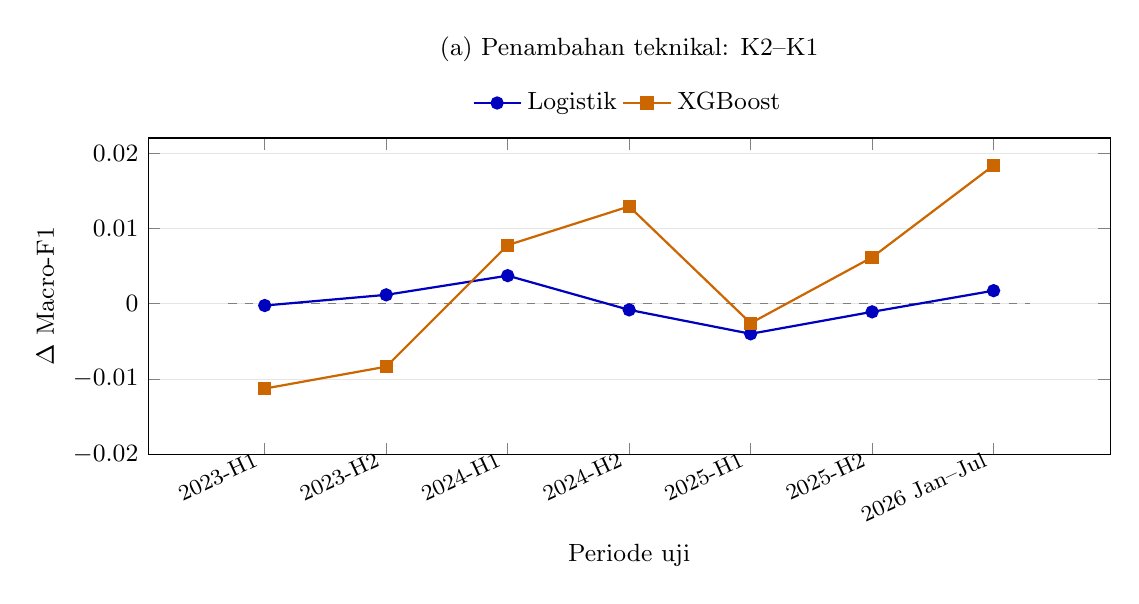
\begin{tikzpicture}
\begin{axis}[
width=13.8cm,height=5.6cm,
font=\small, title style={yshift=1.8em}, title={(a) Penambahan teknikal: K2--K1},
xlabel={Periode uji},ylabel={$\Delta$ Macro-F1},
ymin=-0.020,ymax=0.022,ytick={-0.02,-0.01,0,0.01,0.02},
xtick={0,1,2,3,4,5,6},
xticklabels={2023-H1,2023-H2,2024-H1,2024-H2,2025-H1,2025-H2,2026 Jan--Jul},
x tick label style={rotate=25,anchor=east,font=\footnotesize},
ymajorgrids=true,grid style={gray!20},
legend style={at={(0.5,1.04)},anchor=south,legend columns=2,draw=none,font=\small},
scaled y ticks=false,y tick label style={/pgf/number format/fixed,/pgf/number format/precision=2},
]
\addplot[gray,dashed,forget plot] coordinates {(-0.3,0) (6.3,0)};
\addplot[color=blue!75!black,mark=*,thick] coordinates {(0,-0.000237308407) (1,0.001179526437) (2,0.003726554034) (3,-0.000815538988) (4,-0.003993683096) (5,-0.001076196564) (6,0.001733377549)};
\addlegendentry{Logistik}
\addplot[color=orange!80!black,mark=square*,thick] coordinates {(0,-0.011264536589) (1,-0.008352686929) (2,0.007776872361) (3,0.012919193679) (4,-0.002581653699) (5,0.006162663646) (6,0.018360635190)};
\addlegendentry{XGBoost}
\end{axis}
\end{tikzpicture}

\par\vspace{0.25cm}

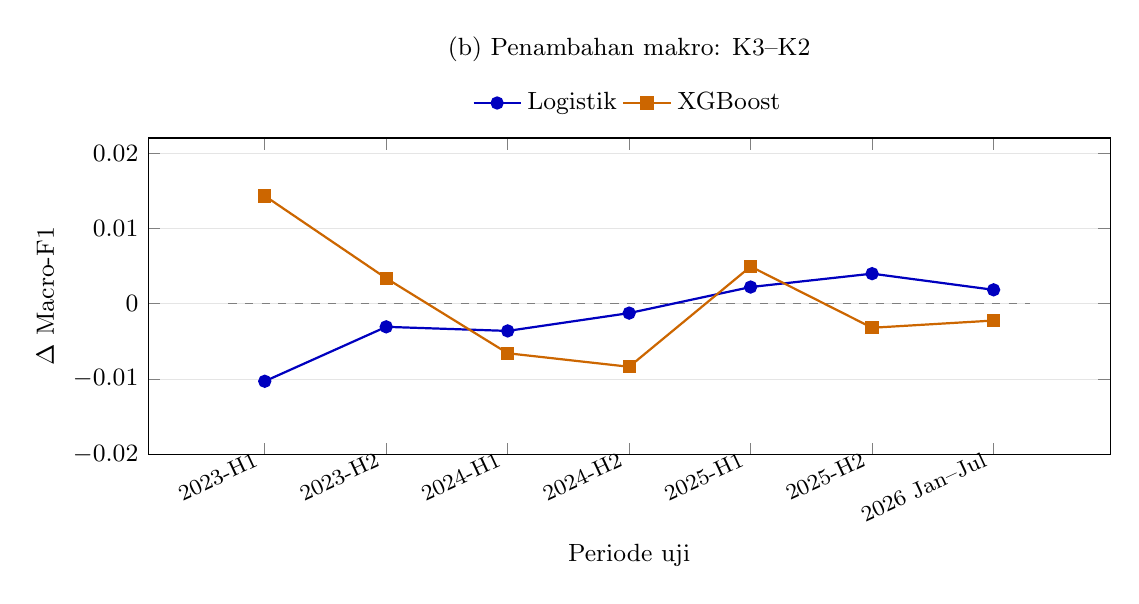
\begin{tikzpicture}
\begin{axis}[
width=13.8cm,height=5.6cm,
font=\small, title style={yshift=1.8em}, title={(b) Penambahan makro: K3--K2},
xlabel={Periode uji},ylabel={$\Delta$ Macro-F1},
ymin=-0.020,ymax=0.022,ytick={-0.02,-0.01,0,0.01,0.02},
xtick={0,1,2,3,4,5,6},
xticklabels={2023-H1,2023-H2,2024-H1,2024-H2,2025-H1,2025-H2,2026 Jan--Jul},
x tick label style={rotate=25,anchor=east,font=\footnotesize},
ymajorgrids=true,grid style={gray!20},
legend style={at={(0.5,1.04)},anchor=south,legend columns=2,draw=none,font=\small},
scaled y ticks=false,y tick label style={/pgf/number format/fixed,/pgf/number format/precision=2},
]
\addplot[gray,dashed,forget plot] coordinates {(-0.3,0) (6.3,0)};
\addplot[color=blue!75!black,mark=*,thick] coordinates {(0,-0.010293657331) (1,-0.003067441448) (2,-0.003609514790) (3,-0.001243463415) (4,0.002215914534) (5,0.003990983680) (6,0.001845835723)};
\addlegendentry{Logistik}
\addplot[color=orange!80!black,mark=square*,thick] coordinates {(0,0.014318816532) (1,0.003377987405) (2,-0.006573671627) (3,-0.008371057397) (4,0.004938371290) (5,-0.003191020754) (6,-0.002230986516)};
\addlegendentry{XGBoost}
\end{axis}
\end{tikzpicture}

\caption{Perubahan macro-F1 per periode pada konfigurasi utama}
\label{fig:hasil-delta-periode}
\end{figure}

\subsection{Sensitivitas Hiperparameter Tetap}

Dalam analisis pada Tabel \ref{tab:hasil-parameter-tetap}, parameter K1 terpilih dipakai kembali pada K2 dan K3 pada periode serta model yang sama. Praproses tetap dipelajari dari data latih untuk konfigurasi terkait. Pada macro-F1, rerata K2--K1 menjadi +0,000285 untuk Regresi Logistik dan $-0{,}001398$ untuk XGBoost. Rerata K3--K2 menjadi $-0{,}001669$ dan +0,003859. Dengan demikian, arah rerata K2--K1 XGBoost pada analisis ini berbeda dari arah rerata perbandingan utama. Kedua analisis dilaporkan terpisah sesuai desain Bab 3.


\begin{table}[htbp]
\centering
\small
\setlength{\tabcolsep}{4pt}
\caption{Perubahan kinerja dengan hiperparameter K1 tetap pada tujuh pasangan utama}
\label{tab:hasil-parameter-tetap}
\begin{tabular}{lllrrrc}
\toprule
Model & Pasangan & Metrik & Rerata & Median & SD sampel & Positif \\
\midrule
Logistik & $K2-K1$ & Macro-F1 & +0,000285 & +0,000546 & 0,002525 & 4/7 \\
Logistik & $K2-K1$ & BA & +0,000430 & +0,000471 & 0,002516 & 6/7 \\
Logistik & $K3-K2$ & Macro-F1 & -0,001669 & -0,001487 & 0,003744 & 3/7 \\
Logistik & $K3-K2$ & BA & -0,000678 & +0,000353 & 0,003387 & 4/7 \\
XGBoost & $K2-K1$ & Macro-F1 & -0,001398 & +0,001720 & 0,006320 & 4/7 \\
XGBoost & $K2-K1$ & BA & -0,001361 & +0,000547 & 0,006196 & 4/7 \\
XGBoost & $K3-K2$ & Macro-F1 & +0,003859 & +0,003469 & 0,007502 & 5/7 \\
XGBoost & $K3-K2$ & BA & +0,004743 & +0,005468 & 0,007674 & 5/7 \\
\bottomrule
\end{tabular}
\end{table}


\section{Hasil Analisis Sensitivitas}

Tabel \ref{tab:hasil-sensitivitas-teknikal} dan Tabel \ref{tab:hasil-sensitivitas-makro} merangkum perubahan macro-F1 untuk seluruh kombinasi sumber, kebijakan celah, dan ambang yang ditetapkan sebelum skor dibaca. Setiap konfigurasi pada kedua tabel memperoleh penyetelan hiperparameter sendiri sebagaimana analisis utama. Kolom ``Pos.'' menyatakan jumlah pasangan dengan selisih positif dibagi jumlah pasangan sah, sedangkan kolom ``Pas./7'' mempertahankan penyebut tujuh periode terjadwal. Singkatan MQ menunjuk MetaQuotes dan U menunjuk Ultima. Kebijakan HR menunjuk \emph{holiday-reset}; P menunjuk primer. Pengali $\alpha$ membentuk ambang $\alpha\sigma_{t,24}$.

Pada sumber MetaQuotes, rerata perubahan K2--K1 Regresi Logistik positif pada kedua kebijakan untuk ambang 0,25 dan 0,50, tetapi pada ambang 1,00 tandanya berbeda antarkebijakan. Untuk XGBoost, tandanya juga berubah menurut ambang dan kebijakan. Pada K3--K2, Regresi Logistik memperoleh rerata negatif pada kelima kombinasi MetaQuotes dan positif pada HR dengan ambang 1,00. XGBoost memperoleh rerata positif pada empat kombinasi MetaQuotes dan negatif pada dua kombinasi. Ringkasan tersebut melaporkan arah yang teramati tanpa mengganti ambang atau kebijakan utama.


\begingroup
\small
\setlength{\tabcolsep}{4pt}
\begin{longtable}{lccrcrcc}
\caption{Sensitivitas rerata perubahan macro-F1 K2--K1}\label{tab:hasil-sensitivitas-teknikal}\\
\toprule
Sumber & Keb. & $\alpha$ & $\Delta$ Logistik & Pos. & $\Delta$ XGBoost & Pos. & Pas./7 \\
\midrule
\endfirsthead
\caption[]{Sensitivitas rerata perubahan macro-F1 K2--K1 (lanjutan)}\\
\toprule
Sumber & Keb. & $\alpha$ & $\Delta$ Logistik & Pos. & $\Delta$ XGBoost & Pos. & Pas./7 \\
\midrule
\endhead
\midrule
\multicolumn{8}{r}{Bersambung ke halaman berikutnya} \\
\endfoot
\endlastfoot
MQ & P & 0,25 & +0,003388 & 6/7 & +0,000844 & 2/7 & 7/7 \\
MQ & P & 0,50 & +0,000074 & 3/7 & +0,003289 & 4/7 & 7/7 \\
MQ & P & 1,00 & +0,000597 & 3/7 & -0,001379 & 3/7 & 7/7 \\
MQ & HR & 0,25 & +0,003886 & 5/7 & -0,004090 & 1/7 & 7/7 \\
MQ & HR & 0,50 & +0,000127 & 5/7 & +0,000366 & 3/7 & 7/7 \\
MQ & HR & 1,00 & -0,000996 & 1/7 & +0,004996 & 5/7 & 7/7 \\
U & P & 0,25 & +0,001906 & 2/4 & +0,007313 & 4/4 & 4/7 \\
U & P & 0,50 & +0,000325 & 3/4 & +0,002690 & 3/4 & 4/7 \\
U & P & 1,00 & -0,000988 & 2/4 & -0,002315 & 2/4 & 4/7 \\
U & HR & 0,25 & +0,000438 & 3/4 & +0,006806 & 2/4 & 4/7 \\
U & HR & 0,50 & -0,001649 & 2/4 & +0,000146 & 3/4 & 4/7 \\
U & HR & 1,00 & -0,000451 & 2/4 & +0,006385 & 3/4 & 4/7 \\
\bottomrule
\end{longtable}
\endgroup


\begingroup
\small
\setlength{\tabcolsep}{4pt}
\begin{longtable}{lccrcrcc}
\caption{Sensitivitas rerata perubahan macro-F1 K3--K2}\label{tab:hasil-sensitivitas-makro}\\
\toprule
Sumber & Keb. & $\alpha$ & $\Delta$ Logistik & Pos. & $\Delta$ XGBoost & Pos. & Pas./7 \\
\midrule
\endfirsthead
\caption[]{Sensitivitas rerata perubahan macro-F1 K3--K2 (lanjutan)}\\
\toprule
Sumber & Keb. & $\alpha$ & $\Delta$ Logistik & Pos. & $\Delta$ XGBoost & Pos. & Pas./7 \\
\midrule
\endhead
\midrule
\multicolumn{8}{r}{Bersambung ke halaman berikutnya} \\
\endfoot
\endlastfoot
MQ & P & 0,25 & -0,000506 & 4/7 & -0,000782 & 3/7 & 7/7 \\
MQ & P & 0,50 & -0,001452 & 3/7 & +0,000324 & 3/7 & 7/7 \\
MQ & P & 1,00 & -0,002087 & 2/7 & +0,006069 & 5/7 & 7/7 \\
MQ & HR & 0,25 & -0,000692 & 3/7 & +0,002305 & 5/7 & 7/7 \\
MQ & HR & 0,50 & -0,000310 & 3/7 & +0,003173 & 4/7 & 7/7 \\
MQ & HR & 1,00 & +0,001001 & 4/7 & -0,001688 & 3/7 & 7/7 \\
U & P & 0,25 & +0,004383 & 3/4 & +0,004089 & 3/4 & 4/7 \\
U & P & 0,50 & +0,004783 & 3/4 & +0,000649 & 2/4 & 4/7 \\
U & P & 1,00 & -0,001029 & 2/4 & +0,007540 & 3/4 & 4/7 \\
U & HR & 0,25 & +0,004950 & 4/4 & +0,002498 & 2/4 & 4/7 \\
U & HR & 0,50 & +0,004385 & 2/4 & +0,004945 & 2/4 & 4/7 \\
U & HR & 1,00 & +0,000507 & 2/4 & -0,000024 & 2/4 & 4/7 \\
\bottomrule
\end{longtable}
\endgroup


Pada sumber Ultima, hasil utama kebijakan primer untuk empat periode sah ditunjukkan pada Tabel \ref{tab:hasil-ultima-rerata}. Rerata macro-F1 K2--K1 positif pada kedua model, sedangkan K3--K2 masing-masing +0,004783 dan +0,000649. Tabel sensitivitas menunjukkan bahwa arah tersebut tidak bertahan pada seluruh pengali ambang dan kebijakan. Hasil Ultima selalu berasal dari empat pasangan sah dari tujuh periode terjadwal, sehingga tidak mempunyai cakupan waktu uji yang sama dengan ringkasan tujuh periode MetaQuotes.


\begin{table}[htbp]
\centering
\small
\setlength{\tabcolsep}{4pt}
\caption{Rerata kinerja Ultima pada kebijakan primer dan ambang utama}
\label{tab:hasil-ultima-rerata}
\begin{tabular}{lcrrc}
\toprule
Model & Konfigurasi & Macro-F1 & Balanced accuracy & Periode sah \\
\midrule
Logistik & K1 & 0,380734 & 0,387797 & 4/7 \\
Logistik & K2 & 0,381058 & 0,388428 & 4/7 \\
Logistik & K3 & 0,385841 & 0,389725 & 4/7 \\
XGBoost & K1 & 0,380839 & 0,382839 & 4/7 \\
XGBoost & K2 & 0,383529 & 0,385571 & 4/7 \\
XGBoost & K3 & 0,384178 & 0,385436 & 4/7 \\
\bottomrule
\end{tabular}
\end{table}


\section{Ketertelusuran dan Batas Hasil yang Dilaporkan}

Konfigurasi, manifes lingkungan, batas periode, dan artefak fitur dibekukan sebelum pembacaan skor utama. Setiap run menyimpan prediksi per bar, label benar, parameter terpilih, kegagalan kandidat, matriks kebingungan, serta checksum. Pemeriksaan ulang pada 2 Oktober 2026 terhadap dua belas run lengkap K1/K2/K3 memastikan checksum prediksi cocok, metrik dapat dihitung ulang dari prediksi, horizon label tidak melewati batas akhir periode uji, dan K1/K2/K3 menggunakan waktu keputusan serta label uji yang sama. Pemeriksaan ini membaca artefak tersimpan tanpa melatih ulang model atau mengganti protokol. Rerun deterministik yang telah tercatat untuk periode 2023-H1 juga menghasilkan prediksi yang identik dengan run lengkap terkait.

Tabel bab ini ditautkan ke ringkasan ber-hash dalam manifes hasil naskah. Hasil utama memiliki tujuh periode sah; sensitivitas Ultima mempertahankan tiga periode awal sebagai \textbf{NOT TESTED}. K3 tetap dibatasi oleh kalender retrospektif tanpa riwayat revisi independen. Ringkasan berpasangan bersifat deskriptif: simpangan baku dan jumlah periode positif menggambarkan variasi hasil yang tersedia, tanpa uji signifikansi yang mengasumsikan periode saling independen.
